% Préambule commun aux manuels de SudokuSolver (français et anglais), au
% format maison des PDF : Latin Modern, titres sans-serif colorés (sky pour
% les sections, alert pour les sous-sections), encadrés tcolorbox, icônes
% fontawesome, anti-titres orphelins, page de garde avec le logo.
% Compilation : python3 docs/src/compiler.py (depuis la racine du dépôt).
\documentclass[11pt,a4paper]{article}
\usepackage[utf8]{inputenc}
\usepackage[T1]{fontenc}
\usepackage{lmodern}
\usepackage{microtype}
\usepackage[a4paper,margin=2cm,headheight=24pt]{geometry}
\usepackage{graphicx}
\usepackage[table]{xcolor}
\usepackage[most]{tcolorbox}
\usepackage{enumitem}
\usepackage{booktabs}
\usepackage{array}
\usepackage{tabularx}
\usepackage[nobottomtitles*]{titlesec}
\usepackage{needspace}
\usepackage{fancyhdr}
\usepackage{fontawesome5}
\usepackage{etoolbox}
\usepackage{listings}
\usepackage{amssymb}
\usepackage[colorlinks=true,linkcolor=sky,urlcolor=sky]{hyperref}
\graphicspath{{../captures/}{../../}}
\input{version}

\definecolor{sky}{HTML}{1C6DB4}
\definecolor{skyl}{HTML}{E6F0F9}
\definecolor{alert}{HTML}{B5382B}
\definecolor{alertl}{HTML}{FBEAE8}
\definecolor{steppe}{HTML}{C08A2E}
\definecolor{steppel}{HTML}{FBF1DC}
\definecolor{summit}{HTML}{6B7A8F}
\definecolor{night}{HTML}{232A56}
\definecolor{ink}{HTML}{1F2430}
\definecolor{codegray}{HTML}{2B2B2B}
\AtBeginDocument{\color{ink}}
% Noms de couleurs de l'ancien manuel, ramenés à la palette maison
\colorlet{darkblue}{night}
\colorlet{midblue}{sky}
\colorlet{lightblue}{skyl}
\colorlet{accent}{steppe}
\definecolor{success}{HTML}{2E7D5B}
\colorlet{danger}{alert}
\definecolor{softgray}{HTML}{F6F6F6}

\titleformat{\section}
  {\Large\bfseries\sffamily\color{sky}}
  {\thesection}{0.6em}{}
  [{\vspace{1pt}\color{sky!35}\titlerule[1.3pt]}]
\titlespacing*{\section}{0pt}{16pt}{8pt}
\titleformat{\subsection}{\large\bfseries\sffamily\color{alert}}{\thesubsection}{0.5em}{}
\titlespacing*{\subsection}{0pt}{12pt}{4pt}
\titleformat{\subsubsection}{\normalsize\bfseries\sffamily\color{night}}{\thesubsubsection}{0.5em}{}
\pretocmd{\section}{\needspace{12\baselineskip}}{}{}
\pretocmd{\subsection}{\needspace{6\baselineskip}}{}{}
\widowpenalty=10000
\clubpenalty=10000
\raggedbottom
\setlength{\parindent}{0pt}
\setlength{\parskip}{6pt}
\setlist{topsep=3pt,itemsep=2pt}

\pagestyle{fancy}
\fancyhf{}
\renewcommand{\headrulewidth}{0.4pt}
\renewcommand{\headrule}{\hbox to\headwidth{\color{sky!40}\leaders\hrule height \headrulewidth\hfill}}
\fancyhead[L]{\sffamily\small\color{sky}\textbf{SudokuSolver} \color{summit}\textbar{} \MANUELTITRE}
\fancyhead[R]{\sffamily\small\color{summit}\thepage}
\fancyfoot[C]{\sffamily\scriptsize\color{summit}Version \VERSIONAPP{} \textbar{} github.com/ARP273-ROSE/SudokuSolver}

\newcommand{\menu}[1]{\textsf{\textbf{\textcolor{sky}{#1}}}}
\newcommand{\touche}[1]{\tcbox[on line,boxsep=0pt,left=2pt,right=2pt,top=1.5pt,bottom=1.5pt,
  colback=white,colframe=summit,boxrule=0.5pt,arc=1.5pt]{\footnotesize\textsf{#1}}}
\newcommand{\fichier}[1]{\texttt{\small #1}}
\newcommand{\capture}[2][1]{\par\needspace{12\baselineskip}\begin{center}\setlength{\fboxsep}{0pt}\setlength{\fboxrule}{0.6pt}%
  \fcolorbox{summit!50}{white}{\includegraphics[width=\dimexpr#1\linewidth-1.3pt\relax]{#2}}\end{center}}

% Deux captures côte à côte, chacune avec sa légende, jamais séparées
\newcommand{\deuxcaptures}[4]{\par\needspace{22\baselineskip}\begin{center}\setlength{\fboxsep}{0pt}\setlength{\fboxrule}{0.6pt}%
  \begin{minipage}[t]{0.47\linewidth}\centering\fcolorbox{summit!50}{white}{\includegraphics[width=\dimexpr\linewidth-1.3pt\relax]{#1}}\\[3pt]{\small\sffamily\color{summit}#2}\end{minipage}\hfill
  \begin{minipage}[t]{0.47\linewidth}\centering\fcolorbox{summit!50}{white}{\includegraphics[width=\dimexpr\linewidth-1.3pt\relax]{#3}}\\[3pt]{\small\sffamily\color{summit}#4}\end{minipage}\end{center}}

% Encadrés (mêmes noms et signatures que l'ancien manuel)
\newtcolorbox{infobox}[1][]{enhanced,unbreakable,colback=skyl,colframe=sky,boxrule=0.9pt,arc=2.5pt,
  left=2.5mm,right=2.5mm,top=1.5mm,bottom=1.5mm,borderline west={2.5pt}{-2.5pt}{sky},#1}
\newtcolorbox{tipbox}[2][]{enhanced,unbreakable,colback=steppel,colframe=steppe!85!black,
  coltitle=white,fonttitle=\bfseries\sffamily\small,boxrule=0.9pt,arc=2.5pt,
  left=2.5mm,right=2.5mm,top=1.5mm,bottom=1.5mm,title={\faLightbulb~~#2},#1}
\newtcolorbox{warnbox}[2][]{enhanced,unbreakable,colback=alertl,colframe=alert,
  coltitle=white,fonttitle=\bfseries\sffamily\small,boxrule=0.9pt,arc=2.5pt,
  left=2.5mm,right=2.5mm,top=1.5mm,bottom=1.5mm,title={\faExclamationTriangle~~#2},#1}

\lstset{basicstyle=\ttfamily\small\color{white},backgroundcolor=\color{codegray},
  frame=single,framerule=0pt,rulecolor=\color{codegray},xleftmargin=6pt,xrightmargin=6pt,
  framexleftmargin=6pt,framexrightmargin=6pt,aboveskip=6pt,belowskip=6pt,
  breaklines=true,showstringspaces=false,
  literate={é}{{\'e}}1 {è}{{\`e}}1 {à}{{\`a}}1 {ê}{{\^e}}1 {ç}{{\c c}}1}

\newcommand{\pagedegarde}[2]{%
  \begin{titlepage}
  \thispagestyle{empty}
  \vspace*{1.4cm}
  \begin{center}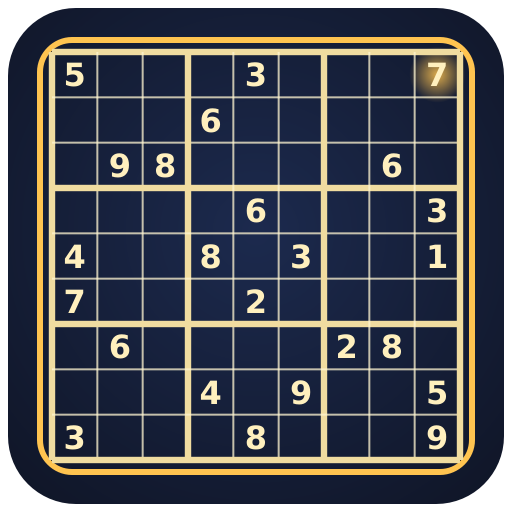
\includegraphics[width=4.4cm]{logo_512.png}\end{center}
  \vspace{8mm}
  {\sffamily\color{summit}\large SudokuSolver\par}
  \vspace{4mm}
  {\color{sky!35}\hrule height 2pt}
  \vspace{7mm}
  {\sffamily\bfseries\color{sky}\fontsize{26}{30}\selectfont #1\par}
  \vspace{4mm}
  {\sffamily\color{night}\large #2\par}
  \vspace{7mm}
  {\color{sky!35}\hrule height 2pt}
  \vspace{5mm}
  {\sffamily\color{summit}\normalsize Version \VERSIONAPP\par}
  \vfill
  {\sffamily\small\color{summit} MIT \textbar{} github.com/ARP273-ROSE/SudokuSolver\par}
  \end{titlepage}}
